\documentclass[
a4paper, 
%a5paper,
%10pt,
%11pt,
12pt,
%twoside, % single sided printout
%oneside, % duplex printout (default)
%% binding correction is used to compensate for the paper lost during binding
%% of the document
%BCOR=0.7cm, % binding correction
%nobcorignoretitle, % do not ignore BCOR for title page
%% the following two options only concern the graphics included by the document
%% class
%grayscaletitle, % keep the title in grayscale
grayscalebody, % keep the rest of the document in grayscale
abstract=on,
%% expert options: your mileage may vary
%baseclass=scrreprt % special option to use a different document baseclass
twoside, BCOR10mm, 12pt, DIV13,headinclude, footexclude, final, abstracton, openright
]{ibireprt}


\usepackage[utf8]{inputenc}
%\usepackage[latin1]{inputenc}
\usepackage[T1]{fontenc}
%\usepackage{ngerman}
\usepackage[ngerman]{babel} %english,


%\usepackage{fancyhdr}
%%\pagestyle{fancy}
%%\lhead{\leftmark}
%\fancyhead[OR]{\thepage}% ungerade Seiten, rechts \thepage
%\fancyhead[OL]{\leftmark}% ungerade Seiten, links
%\fancyhead[ER]{\leftmark}% gerade Seiten, rechts
%\fancyhead[EL]{\thepage}% gerade Seiten, links \thepage
%\cfoot{}
%\pagestyle{fancy}

\renewcommand{\chaptermark}[1]{\markboth{#1}{}}
\renewcommand{\sectionmark}[1]{\markright{#1}{}}

\setlength{\parindent}{0em}
%\setlength{\parskip}{0mm}
\setcounter{tocdepth}{1}
\setcounter{secnumdepth}{2}
%\linespread{1.15}

\usepackage{quotchap}
\usepackage{nccmath}

\usepackage{microtype}

\usepackage{qtxmath,tgtermes}
\usepackage[scaled=.90]{helvet}
\usepackage{courier}

\usepackage{graphicx}
\usepackage{amsmath}
%\usepackage{amsfonts}
\usepackage{amssymb}
\usepackage{tabularx}
%\usepackage[bookmarks,plainpages=false]{hyperref} %colorlinks  ,urlbordercolor={111},linkbordercolor={111},citebordercolor={111}
\usepackage[Algorithmus]{algorithm}
\usepackage{algorithmic}
%\usepackage{tkmath}
\usepackage{exscale}
\usepackage{empheq}
\usepackage{color}
\usepackage{framed}
\usepackage{rotating}
\usepackage{longtable}
\usepackage[hang,small,bf]{caption}
\usepackage{booktabs}
\usepackage{colortbl}

\usepackage[babel,german=quotes]{csquotes}
\usepackage{ntheorem}
\usepackage{blindtext}

%\mathindent1.5cm
\def\fleq{\@fleqntrue \let\mathindent\@mathmargin \@mathmargin=\leftmargini}
\def\cneq{\@fleqnfalse}


%\setcapindent{0em}

\newenvironment{fshaded}{%
\def\FrameCommand{\fcolorbox{framecolor}{shadecolor}}%
\MakeFramed {\FrameRestore}}%
{\endMakeFramed}

\theoremseparator{:}

\newtheorem{theorem}{Theorem}[chapter]
\newtheorem{lemma}{Lemma}[chapter]
\newtheorem{remark}[theorem]{Bemerkung}
\newtheorem{definition}[theorem]{Definition}
\newtheorem{example}{Beispiel}
%\newtheorem{proof}[theorem]{Beweis}
\newtheorem{corollary}[theorem]{Corollary}

\newenvironment{Theorem}{\goodbreak \definecolor{shadecolor}{rgb}{0.95,0.95,0.95}%
\definecolor{framecolor}{rgb}{0,0,0}%
\begin{fshaded}\begin{theorem}\sl}{\end{theorem} \end{fshaded}}
\newenvironment{Lemma}{\goodbreak \definecolor{shadecolor}{rgb}{0.95,0.95,0.95}%
\definecolor{framecolor}{rgb}{0,0,0}%
\begin{fshaded} \begin{lemma}\sl}{\end{lemma} \end{fshaded}}
\newenvironment{Remark}{\goodbreak \begin{remark}\rm}{\hfill  $\square$\end{remark}}
\newenvironment{Example}{\goodbreak \begin{example}\rm}{\hfill $\square$ \end{example}}
%\newenvironment{Proof}{\goodbreak \begin{proof}\rm}{\hfill $\blacksquare$ \end{proof}}
\newenvironment{Definition}{\goodbreak \definecolor{shadecolor}{rgb}{0.95,0.95,0.95}%
\definecolor{framecolor}{rgb}{0,0,0}%
\begin{fshaded} \begin{definition}\rm}{\hfill  \end{definition} \end{fshaded} }
\newenvironment{Corollary}{\goodbreak \begin{corollary}\rm}{\end{corollary}}

\newenvironment{Proof}[1][Beweis:]{\begin{trivlist}
\item[\hskip \labelsep {\bfseries #1}]}{\hfill $\blacksquare$\end{trivlist}}

\numberwithin{equation}{chapter}
\numberwithin{table}{chapter}
\numberwithin{figure}{chapter}
\numberwithin{algorithm}{chapter}
\numberwithin{example}{chapter}
\numberwithin{example}{chapter}

\def\i{\mbox{\small{\rm i}}}
\def\ti{\mbox{\scriptsize{\rm i}}}
\newcommand{\e}[1]{{\rm e}^{ #1}}
\renewcommand{\mod}{\;{\rm mod}\;}

\newcommand{\zb}[1]{\mbox{\boldmath{${#1}$}}}
\newcommand{\zbs}[1]{\mbox{\boldmath\scriptsize{${#1}$}}}
\newcommand{\zbss}[1]{\mbox{\boldmath\tiny{${#1}$}}}

\newcommand{\adj}{{\ensuremath{\mathsf{H}}}}
\newcommand{\trans}{{\ensuremath{\mathsf{T}}}}


% Keine "Schusterjungen"
\clubpenalty = 10000
% Keine "Hurenkinder"
\widowpenalty = 10000 \displaywidowpenalty = 10000 %\displaywidowpenalty = 10000






% Information for the Titlepage
\author{Johann Strunck}
\title{Deep learning based grading of motionartifacts in HR-pQCT}
%\date{\today}
\date{\today}
\subject{Bachelor thesis}
\professor{Prof.~Dr.-Ing.~Tobias Knopp}
\advisor{Dr.~rer.~nat.~Martin Hofmann}







\begin{document}
%\frontmatter
\maketitle
%\mainmatter


\newpage
${}^{}$
\vfill
\noindent
Ich versichere an Eides statt, die vorliegende Arbeit selbstständig und nur unter Benutzung der angegebenen Quellen und Hilfsmittel angefertigt zu haben.\\
\vspace{1.5cm}

\noindent
Hamburg, den ??.??.2010
\thispagestyle{empty}
\newpage
\newpage

\setlength{\parskip}{1.5mm }

%\newpage

%\maketitle



\tableofcontents


\chapter*{Summary}
	In the research field of osteoporosis High-resolution peripheral quantitative computed tomography (HR-pQCT) scans are used to ...%TODO: this part needs to be added otherwise it sounds bland
	
	
	A common issue of HR-pQCT scans is the appearance of motion artifacts in Images. These artifacts can appear due to involuntary movements like twitches and spasms. Since a scan can last between 3-4 minutes its hard not to move for such a long time. Depending on the severeness of those artifacts in the resulting image, it might not be sufficient for medical use and a re scan is necessary. The decision of the severity is made by a qualified person which gives the image a number from 1 to 5, where 1 equals no motion artifacts and 5 equals severe motion artifacts. The decision of severity is a  biased process and the score varies depending on the reviewing person. Studies showed that operators disagree in up to 30\% %TODO: find wich paper this was and include it
	of all cases where a re scan might or might not be necessary. This findings also match with our data, since we also have a disagreement in around 30\% of all cases. To support the decision of the operators there have been approaches by \cite{Sode2011} and \cite{Walle2023}  to improve the confidence of the result. both methods can be performed with the absence of a operator and results of \cite{Sode2011} show that with cross validation of a operator  a Convolutional Neural Network(CNN) can reach a higher accuracy than the cross validation of two operators without a CNN. The CNN still has a considerable error rate. In this paper we will propose a new CNN structure which uses state of the art methods to detect the severity of motion Scores in CT scans. %TODO: the evaluation of the findings still needs to be written this can just be done when the paper is finished

\chapter{Introduction}

High-resolution peripheral quantitative computed tomography (HR-pQCT) is a specialized non-invasive imaging technique that provides detailed and accurate three-dimensional images of bone and tissue micro architecture at the peripheral skeletal sites. In our paper we focus  on the radius and tibia. This advanced imaging technique offers several distinct advantages. One advantage is that HR-pQCT provides high resolution images that allow a thorough assessment of a scanned bone micro architecture. It offers precise measurement of bone mineral density(BMD) and geometric parameters such as trabecular thickness and cortical thickness. HR-pQCT has applications in both clinical and research setting and can help make more informed decisions about patient management and treatment strategies. It can provide insight into fracture or the risk of its occurrence. HR-pQCT imaging requires the patient to remain in position during the scan to avoid motion artifacts. This can be challenging for certain patient populations, such as children or individuals with limited  mobility. The XtremCT (Scanco Media AG), a device that  was used to generated the test and training data for this paper is vulnerable to patient movement it takes about 3-4 Minutes for a scan which makes it hard to hold the chosen extremity in place for such a long time. This is also an issue when the extremity is hold in place by a cast.

 Depending on the severity of the motion artifact the scan must be repeated. To determine the severity of the scan, \cite{Whittier2020} Introduced a scale from 1 (no visible motion artifacts) to 5 (significant horizontal streaks) to grade the severity of motion in scans. In clinical studies it is commonly implemented, that scans with a grading of 4 or 5 have to be repeated to get another scan with possibly mitigated motion artifacts. However, even with a standardized scoring system, motion scoring remains subjective, and operator agreement has shown to remain only moderate, even with intensive training [], studies have shown that operators disagree in up to 30\% of all cases[look at bone]. Due to this issue a objective and standardized method is desirable for the grading process. Papers like \cite{Sode2011} and \cite{Walle2023} have taken an approach to find a suitable method for grading motion artifacts, with partial success.
 
<<<<<<< HEAD
\cite{Walle2023} proposes a method for objective detection of subject motion. The first method measures subject motion by comparing the projections at 0° and 180° since those projections are parallelized, they should be the mirror of each other when no subject motion occurred. Therefore by comparing the difference of those two parallel projections the subject motion can be approximated. This method is called Quantitative Motion Estimate(QME) and utilizes a similarity measure like the sum of squared intensity difference(SSD) or normalized cross correlation (NCC) to compare the mirrored parallel projection image at 0° and 180°.% TODO: way to deteailed remove informations (after second read i actually like it) still tehr needs to be a way to merge this part with the next one  
 %vlt zu konkret das sollte glaube ich eher in die beschreibung der algorithmen rein kommen 
%The main Constrain of this approach is that the subject could move and then land in the same position which would lead to a wrong label.

In the last few years a tremendous interest in machine learning emerged. Many applications have found a way in our modern society \cite{LeCun2015}. They can be found in applications like speech to text or the recommendations on e-commerce websites. The field of medical imaging is no exception to this, including computer aided diagnosis, radiomics, and medical image analysis[]. %TODO: write more to medical imaging
With the emerging field of deep learning in computer vision it became more attention. In 2012 the ILSVRC2012 challange  was won by the CNN based Network AlexNet outperforming the runner up with 10.8 percentage points lower top-5 error score of 15.3\% . Since then the application of deep learning structures like CNNs have seen rapid growth in fields like medical imaging. 

 ...\cite{Yamashita2018} %TODO: look at this paper to write this part another paper is


A frequently occurring issue in medical imaging is the lack of training data. In our case we had 500 labeled examples of tibia and radius.

The data that we use in this paper to compare the different approaches was provided by the Osteology department of the Universitäts Klinikum Eppendorf. All 500 provided scans where generated by the Scanco XtremCT. % maybe explain the basics of ct scans 
To ensure the correctness of the labels, three doctors of the institution labeled the data together to ensure that the data was generalized and therefore reducing the subjective influence of the single person.  

 If we compare the data to the amounts of data used in training state of the art networks like ImageNet with many Million Examples it's a small fraction. This comes on the one hand from the fact that the labeling task in medical imaging can just be performed my professionals and therefore the labeling process is costly and just a few people can do it. Another issue is the availability of data since patient data cant be accessed and used as easy. Therefore we need to find a way to augment the data so that we don't run into problems like overfitting or poor generalization of the network 
=======
\cite{Walle2023} proposes a method for objective detection of subject motion. The first method measures subject motion by comparing the projections at 0° and 180° since those projections are parallelized, the should be the mirror of each other when no subject motion occurred. Therefore by comparing the difference of those two parallel projections the subject motion can be approximated. This method is called Quantitative Motion Estimate and utilizes a similarity measure like the sum of squared intensity difference(SSD) or normalized cross correlation (NCC) to compare the mirrored parallel projection image at 0° and 180°.

In resent years a tremendous intrest in deep learning networks has emerged \cite{LeCun2015} ...\cite{Yamashita2018} %TODO: look at this paper to write this part another paper is
 %vlt zu konkret das sollte glaube ich eher in die beschreibung der algorithmen rein kommen 
  %The main Constrain of this approach is that the subject could move and then land in the same position which would lead to a wrong label.
 
>>>>>>> parent of e570a91 (added a lot of text to the latex file)
  

\cite{Sode2011} uses the power of CNNs to train a network for grading motion artifacts. Deep learning techniques, particularly CNNs, have revolutionized medical image analysis. CNNs are a subset of (ANNs), with each node detecting local features from the input vector, minimizing the parameters in a process called down-sampling, and the subsequent layers combining these features into a fully connected layer.%TODO: rewrite last sentence in own words 

CNNs excel at tasks such as image segmentation, object detection, and classification. With their ability to automatically learn intricate patterns and features from complex visual data, enabling more accurate and efficient diagnostic processes. %more information necessary 
Even with the simplistic structure chosen in \cite{Sode2011} the Network is reaching a accuracy of ..., this can lead to the assumption that a more sophisticated network might be more suitable . In this paper we will build on those findings and try to create a stronger network with state of the art CNN building blocks 


%TODO: part about CNN's
In this paper we will introduce a Convolutional Neural Network Structure which is designed to predict the severity of the motion artifact and compare this Structure to the findings of \cite{Sode2011} and \cite{Walle2023}. 
<<<<<<< HEAD
%TODO: can defenetly be longer 
=======

The data that we use in this paper to compare the different approaches was provided by the "Universitäts Klinikum Eppendorf". All 500 provided scans where generated by the Scanco XtremCT.% maybe explain the basics of ct scans 
to ensure the correctness of the labeled data three doctors of the institution labeled the data together to ensure that the data was generalized and reduce the subjective influence of the single person  
>>>>>>> parent of e570a91 (added a lot of text to the latex file)


A frequently occurring issue in medical imaging is the lack of training data. In our case we had 500 labeled examples of tibia and radius. If we compare this to the amount of data used in training state of the art networks like ImageNet with many Million Examples it's a small fraction. This comes on the one hand from the fact that the labeling task in medical imaging can just be performed my professionals and therefore the labeling process is costly and just a few people can do it. Another issue is the availability of data since patient data cant be accessed and used as easy. Therefore we need to find a way to augment the data so that we don't run into problems like overfitting the Network or poor generalization of the network
\chapter{Literature review}

\begin{figure}[h]	
	\center
	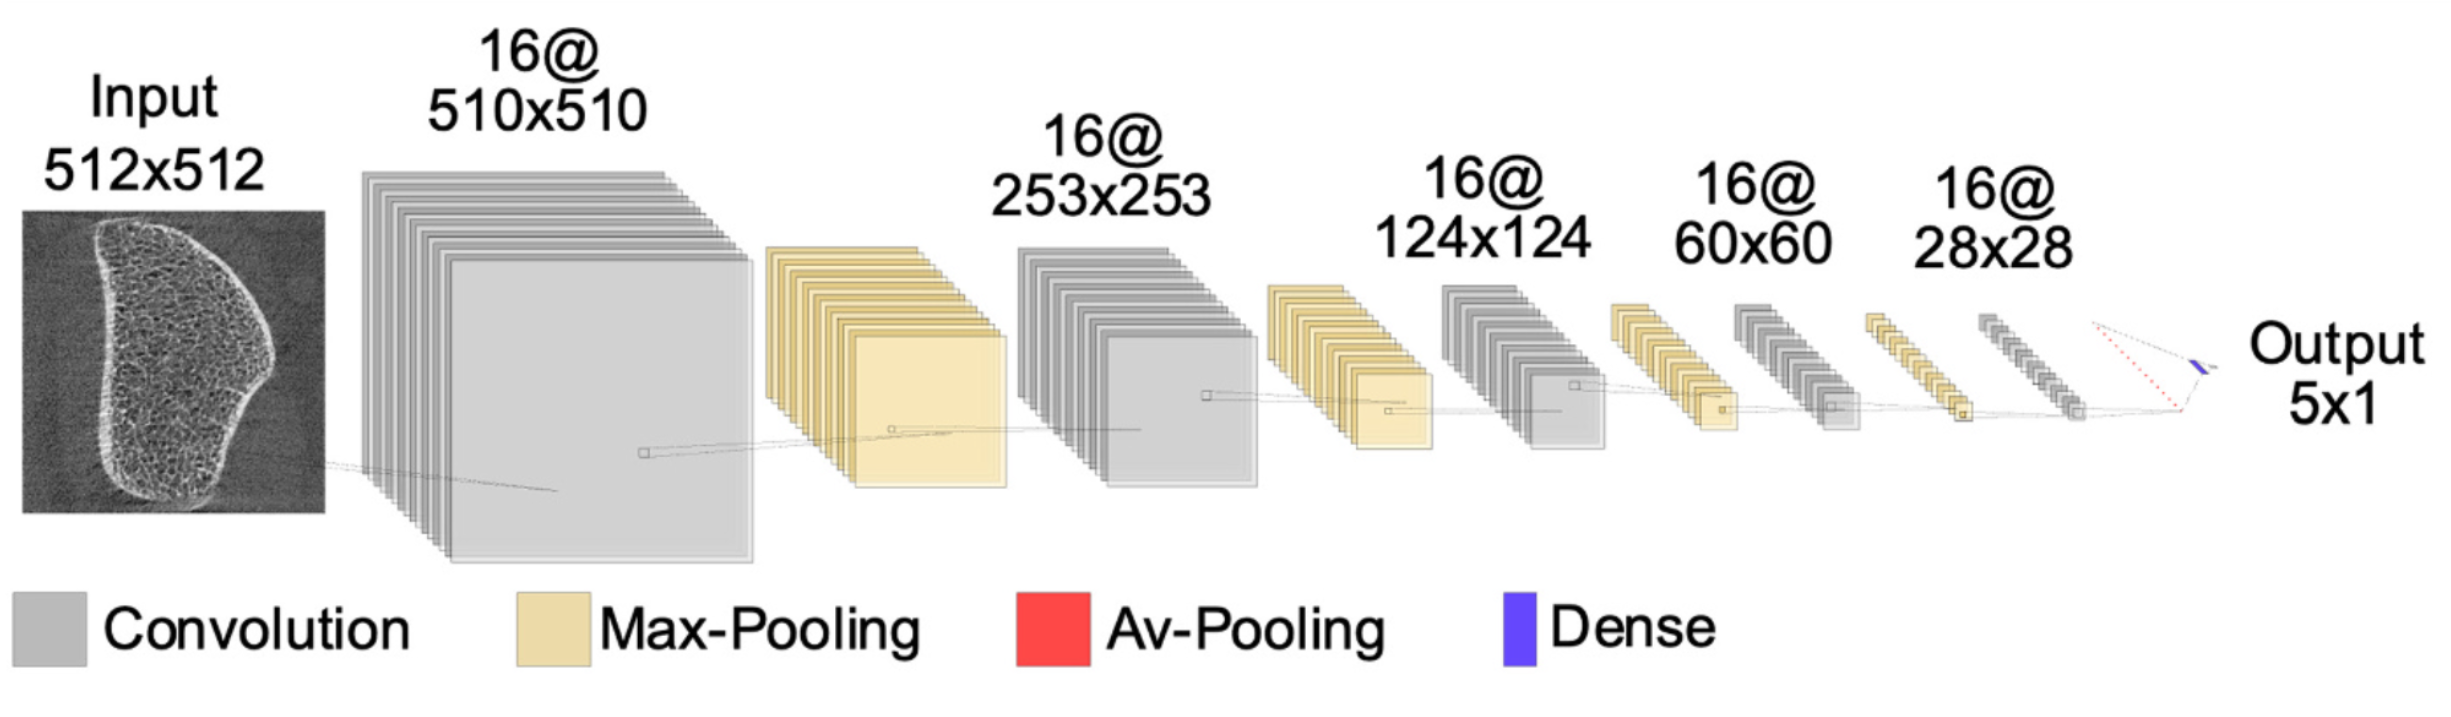
\includegraphics[width = 1 \textwidth]{Bone_Network_Structure.png}%
	\caption{Network Structure Bone}
	\label{fig:fig1}
\end{figure}%

<<<<<<< HEAD
\cite{Walle2023} introduces a CNN which was trained to classify the severity of motion artifacts in HR-pQCT. The Network was trained with images(XtremeCT II, Scanco Media AG) from 90 patients. The size of the scans was 512 x 512 x 168. for the training 8 equally spaced images from every scan were used resulting in a database of 3312 images.
The implemented Network strucuture begins with five alternating convolutional and max-pooling layers followed by a average pooling layer and is concluded by a dense layer. To extract the most important features max Pooling was used followed by a convolutional layer to aggregate them. Convolutional layer used (LeakyReLu) activation to enable faster learning while avoiding dead neurons.
%TODO: aufpassen einfach koppiert vlt umformulieren , außerdem fehlen da echt viele informationen zu den gründen der verwendung der einzelnden layers 
 The classification was performed by a Fully Connected Layer integrating non-linear combinations of all high-level features using a standard Rectified Linear Unit (ReLU) activation function . On the output layer, a Softmax activation function provided an output that may be understood as a class probability, with each output larger than zero and their total always equal to one
%TODO: the text above is way to dense with informations a few filling sentences would it good 
%TODO finis this methode 

\begin{figure}[h]
	\center
	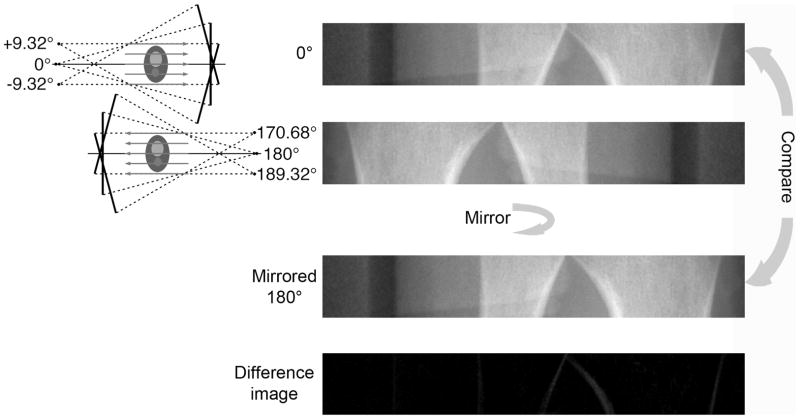
\includegraphics[width = 1 \textwidth]{Sode_rotated_scan.png}[h]%
	\caption{Rotated Scans}
	\label{figure:fig2}
\end{figure}
%TODO: text ist noch nicht unter dem bild das muss geändert werden außerdem ist dieser ganze teil noch rellati nichts sagend es wirkt so alsob informationen fehlen
\cite{Sode2011} introduced a technique to measure the subject motion based on a calculation of the percent  difference in each bone for the paired scans with and without visually apparent motion artifacts. QMEs for each motion degraded scan were calculated using two different image similarity measures: sum of squared differences(SSD) and normalized cross correlation(NCC) which were applied to the projections at 0$^{\circ}$, 0.24$^{\circ}$ and 180$^{\circ}$ since they are  parallelized. The image at 180$^{\circ}$ was then mirrored with respect to the center of rotation on the detector to match the image at 0$^{\circ}$. 
\begin{align}
	SSD = \sum_{i}^{N}(f_i-g_i)^2 \textrm{ and }
	 NCC = \frac{\sum_{i}^{N}(f_i \cdot g_i)}{\sqrt{\sum_{i}^{N}(f_i^2) \cdot \sum_{i}^{N}g_i^2}}
\end{align}

N is the number of voxels and $f_i$ and $g_i$ are the intensity values of the $i$th voxel. The greater the difference of the images, the larger is the SSD and the larger the deviation from 1 for NCC. To account for the bone size, density positioning and other covariables the similarity measure at 0$^{\circ}$ and 180$^{\circ}$ was normalized by the similarity measure of the images at 0$^{\circ}$ and 0.24$^{\circ}$
Therefore the quantitative motion estimates(QMEs) can be calculated by: 
\begin{align}
	QME_{SSD}= \frac{SSD_{0^{\circ} vs 180^{\circ}}}{SSD_{0^{\circ} vs 0.24^{\circ}}} \textrm{ and }	QME_{NCC}=100 \cdot \sqrt{ \frac{NCC_{0^{\circ} vs 180^{\circ}}}{NCC_{0^{\circ} vs 0.24^{\circ}}}}
\end{align}
SSD- and NCC- based QME increases proportionally to the image quality. IT was detected that NCC is most suitable for detecting small affine translation, but is less sensitive to a large translation.%TODO: what does translation mean is it even the right word 

\chapter{Methods}
%CT
%TODO: Anfang fehlt startet zu schnell in das thema 
Computer tomography(CT) uses a three dimensional radiographic imaging technique. The formation process begins with the acquisition of sequential radiographic projections captured over a range of angular positions around the object of interest. The cross sectional field of view is reconstructed using established computational techniques based on the radon projection theory\cite{article}. Similar to simple radiography, the reconstructed image’s intensity values represent the local radiographic attenuation: a material property related to the object’s electron density (atomic number and mass density). The contrast between soft and mineralized tissue in CT is high, due to the relative electron-dense inorganic component (calcium hydroxyapatite) of the bone matrix.These principles capture high-resolution images of bone across a range of structural scales. %TODO: das habe ich koppiert (muss unbedingt  umgeschrieben werden )

%HR-pQCT
High resolution peripheral quantitative computer tomography(HR-pQCT) is a  dedicated extremity imaging system developed to image bone microarchitecture in vivo at peripheral skeletal sites \cite{Bergh2021}. This imaging method gives information on the bone structure and mineral density in bones like radius and tibia. This information allows the estimation of the bone strength and ability to resist fracture. The extraction of this information is possible do due to the high resolution of HR-pQCT.%TODO: how does it achieve the high resolution 
 HR-pQCT is a low radiation dose method, with a effective radiation dose at the distal radius and tibia of  3-5 \textmu SV depending on the scanner  generation. This is significantly less when comparing it to other common medical imaging techniques like chest X-rays with 100\textmu SV or a hip CT scan with 2000-3000 \textmu SV.%TODO: why is it good that it doesnot use as much radiation
  A big field of study using this technique is the field of osteoporosis. Osteoporosis causes bones to become weak and brittle, so brittle that a fall or even mild stresses such as bending over or coughing can cause a fracture. Six individual studies demonstrated that HR-pQCT variables could predict incident fractures in postmenopausal woman and old men, suggesting that the assessment of cortical and trabecular bone microarchitecture by HR-pQCT could improve overall fracture prediction. There are still no widespread use of HR-pQCT since there is just a small number of devices installed(fewer than 100 in mid 2020) therefore the main use of HR-pQCT is related to research \cite{Bergh2021}.


%machine learning 
In the recent years machine learning has become a popular in the research domain due to its versatile nature. It is a branch of artificial intelligence and computer science which focuses on the use of data and algorithms to imitate the way humans learn. A machine learning algorithm operates by processing data to identify patterns and connections. It learns from the data through a training process, adjusting its internal parameters to minimize a measure called "loss". This loss quantifies the difference between the algorithm's predictions and the actual outcomes in the training data. The algorithm iterative refines its parameters to reduce this loss, making its predictions more accurate. Once trained, the algorithm can apply its learning to new, unseen data, aiming to make predictions or classifications with minimized error based on its learned patterns.
%optimizers
The process of refining the data is done by a so called optimizer. There are various different optimization algorithms like stochastic gradient descent, RMSprop, Momentum or Adam. These algorithms differ in how they calculate and apply parameter updates based on the gradients of the loss function with respect to the models parameters (weight and biases) during training. The optimizer  seeks to find the optimal set of parameters by iterative updating the parameters in a way that moves the model in the direction of decreasing loss.

%TODO: write about how it all started with gradient descent and then go on to adam 
Gradient Descent is one of the most common ways to optimize a Neural Network \cite{Ruder2016}. It is a way to minimize a objective function by updating the parameters in the opposite direction of its gradient. There are three different variants of gradient descent that are differing in how much data they use to calculate the gradient of the cost function. There is Stochastic gradient descent, batch gradient descent and mini batch gradient descent. 
%TODO:next part should be structured differently dont start with mini batch gradient descent (baybe just rewrite it and explain every single thing by itselfe might sound better )
Mini batch gradient descent is a compromise between stochastic gradient descent and batch gradient descent since it just takes a small amount of data for calculating the gradient. This is more accurate then stochastic gradient descent since stochastic gradient descent calculates its gradient based on one example, but it isn't as fast. Compared to Batch gradient descent it is faster since Batch gradient descent takes all the examples into account but therefor batch gradient descent is more accurate.Since mini batch gradient descent is a compromise of the other two variants and has a good balance between computation cost and accuracy it is the commonly used gradient descent algoritm. By calculating the gradient of the cost function and subtracting it from ... %TODO: dont really know how to express this
 this is used to find a local minimum of the cost function, sometimes it can even find the global minimum but that is rarely the case. To ensure that the algorithm can find a minimum a learning rate $\eta$ is implemented. This makes it possible that the gradient descent method can come as close to a minimum of the cost function as possible. Even with the adjustment of the learningrate it is nearly impossible to reach the global minima since the learning algorithm usually gets caught in in a local minima or saddle point. %TODO: this can be explained in more detail 
 
\begin{align}
	\theta = \theta - \eta \cdot \nabla_\theta J(\theta)
\end{align}

%TODO: text has some words that are not really scientific
%adaption of the learning rate and global and local minimas 

 Since the developement of gradient descent there has been a lot of progress and new, more efficient algorithms were developed. 



%Adam 
adaptive moment estimation(Adam)\cite{Kingma2014} is a first-order gradient-based optimization technique or learning algortihm that is widely used, representing the latest trend in deep learning optimization. Adam is a deep learning strategy that was specifically designed for training deep neural networks. Its main selling points are it's memory efficiency and less computational cost compared to other optimization algorithms. It  utilizes the squared gradients($v_t$) to scale the learning rate like RMSprop and  is similar to momentum by using the moving average of the gradient($m_t$).%TODO: finde something to cite for momentum and RMSprop and also ad a short explanation of those two algorithms 
%TODO: more text needed to fast transistion to formulas 
\begin{align}
	m_t =\beta_1\cdot m_{t-1} + (1- \beta_1)\cdot g_t \\
	v_t =\beta_2\cdot v_{t-1} + (1- \beta_2)\cdot g_t^2
\end{align}
$m_t$ and $v_t$ are estimates of the first moment (the mean) and the second moment (the uncentered
variance) these moving averages are initialized as vectors of 0's leading to moment estimates that are  biased towards zero. The initialization bias can be counteracted resulting in bias-corrected estimates $\hat{m}_t$ and $\hat{v}_t$

\begin{align}
		\hat{m}_t = m_t/(1- \beta_1^t)\\
	\hat{v}_t = v_t/(1- \beta_2^t)
\end{align}
Those moment estimates can then be used to update the parameters: 
\begin{align}
	\omega_t = \omega_{t-1}-\alpha\cdot\hat{m}(\sqrt{\hat{v}_t}+\epsilon)
\end{align}
Good default settings are stepsize $\alpha = 0.001$, exponential decay rates for the moment estimates $\beta_1 = 0.9 \beta_2 = 0.999 $ and $\epsilon =  10^{-10}$.


%TODO: zu diesem paper kann auch noch mehr geschrieben werden wie zum beispiel das adam keine learning rate braucht sondern sich selbst reguliert und das adam sich glaube ich auch seine richtung korrieigeren kann außerdem muss  w_t erklärt werden

Still using Adam is not sufficient to achieve the best results in the absence of added gradient noise \cite{Neelakantan2015}...%TODO: this paragraph still needs to be written 


%this algorithm is first initialized with random variables which are then 
% those algorithms can be seen as networks of interconnected functions which get a set of data as input to generate a output. This can be seen as a

Before we can train a network we first of all have to initialize the values of all the neurons weights and biases.  
%TODO:need to explain the meaning of neurones this should be done at a earlyer stage with a thourough explanation of basic network structures 

%TODO: do i want to explaing the process of initiallisation and updating the weights and biaseses it might be smart especially because we could then talk about of initializing the parameters maybe even the technique that wete showed.

%TODO: mini batch gradient descent 
=======
Bone et al introduces a CNN in his paper which he trained to classify the severity of motion artifacts in HR-pQCT. He trained his network with images(XtremeCT II, Scanco Media AG) from 90 patients. The size of the scans was 512 x 512 x 168. for the training he used 8 equally spaced images from every scan  resulting in a database of 3312 images.
The implemented Network strucuture begins with five alternating convolutional and max-pooling layers followed by a average pooling layer and is concluded by a dense layer. To extract the most important features max Pooling was used followed by a convolutional layer to aggregate them. Convolutional layer used (LeakyReLu) activation to enable faster learning while avoiding dead neurons.
%aufpassen einfach koppiert vlt umformulieren 
 The classification was performed by a Fully Connected layer r integrating non-linear combinations of all high-level features using a standard Rectified Linear
Unit (ReLU) activation function . On the output layer, a Softmax activation function provided an output that may be understood as a class probability, with each output larger than zero and their total always equal to one

\chapter{Methods}
%CT
Computer tomography(CT) uses a three dimensional radiographic imaging technique. The formation process begins with the acquisition of sequential radiographic projections captured over a range of angular positions around the object of interest. The crossectional field of view is reconstructed using established computational techniques based on the radon projection theory\cite{article}.Similar to simple radiography, the reconstructed image’s intensity values represent the local radiographic attenuation: a material property related to the object’s electron density (atomic number and mass density). The contrast between soft and mineralized tissue in CT is high, due to the relative electron-dense inorganic component (calcium hydroxyapatite) of the bone matrix.These principles capture high-resolution images of bone
across a range of structural scales. %das habe ich koppiert (muss unbedingt umgeschrieben werden )
%HR-pQCT
High resolution peripheral quantitative computer tomography(HR-pQCT) is a  dedicated extremity imaging system designed for trabecular-scale imaging and is currently available from a single manufacturer (XtremeCT; Scanco Medical AG,
Bru¨ttisellen, Switzerland). 

>>>>>>> parent of e570a91 (added a lot of text to the latex file)

%CNN
Convolutional Neural Networks (CNNs) are a class of deep learning models specifically designed for processing structured grid-like data, such as images, by automatically learning hierarchical patterns and features. CNNs are widely used in computer vision tasks and have revolutionized the field of image recognition, object detection, and image generation. CNNs excel at tasks like image classification, where the network assigns a label or category to an input image\\
%Convolutional Layer

The fundamental building blocks of CNNs are convolutional layers, which perform convolution operations on input data. These layers apply a set of learnable filters (also called kernels) to input images by sliding the filter over the input data and computing element-wise multiplications and summations to produce feature maps \ref{fig:fig2}. This layers purpose is detecting different features like edges, textures, and more complex patterns. The learned features become progressively more abstract as they pass through multiple convolutional layers making it possible to classify complex structures.	Two key hyperparameters that define the convolution operation are size and number of kernels. The former is typically 3 × 3, but sometimes 5 × 5 or 7 × 7. The application of a Convolutional layer on a Matrix, shrinks it in size, to mitigate this effect there are two parameters that can be set to get the desirable output size. On the one hand we can add Padding, this adds a number of zero rows and columns to the matrix increasing the output size. During the convolution,the filter slides over the matrix from left to right and top to bottom. Stride is the second changeable parameter. It is defined as the step size of the filter, meaning its the definition of how many elements the filter moves to the right or bottom per iteration.\\%TODO: at the end there could be more sentences to make the text easyer to read 

\begin{figure}[h]
	\center
	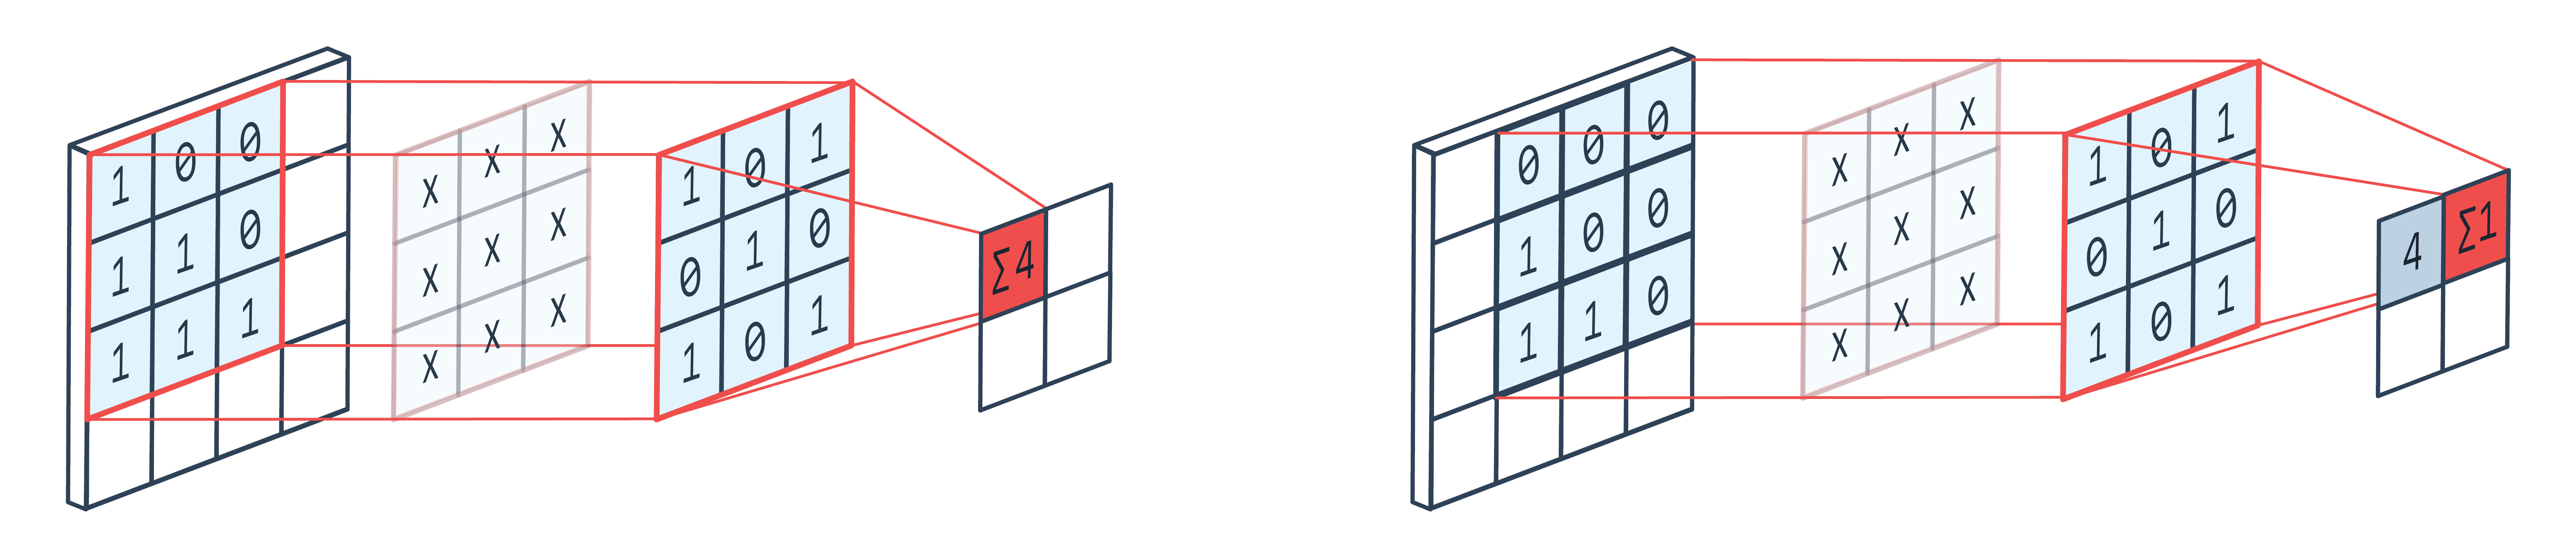
\includegraphics[width = 1 \textwidth]{Conv_Layer.png}%
	\caption{Convolutional Layer with Kernel 3x3}
	\label{fig:fig2}
	%https://datascience.stackexchange.com/questions/80436/understanding-how-convolutional-layers-work
\end{figure}


%Pooling Layer
The Convolutional layer is usually followed by a Pooling layer. This  layers downsample the feature maps, reducing the spatial dimensions while retaining important information.Usually The stride matches the field size of the pooling operation, so that no feature of the previous layer is used twice. Max pooling and average pooling are the most common applied pooling operations. In the Max pooling opperation the maximum value of the current view is selected, this preserves detected features especially the most commonly used ones. The average pooling operation takes the averages of the values of the current view. During training in back propagation average pooling provides a smoother gradient compared to max pooling. It also retains information from the original image since average pooling takes the collective information into account. \\ %TODO:maybe talk about max average pooling and find a better transition to the fc layer
\begin{figure}[h]
	\centering
	\begin{minipage}[t]{.45\linewidth}
		\centering
		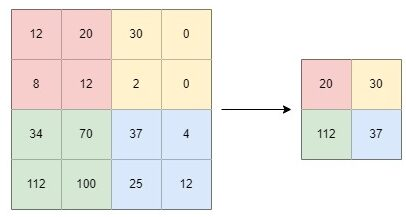
\includegraphics[width = \textwidth]{MaxPooling.jpg}%
		\caption{Max Pooling Layer with Kernel 2x2 and Stride 2}
		\label{fig:fig_max_pooling}
		
	\end{minipage}
	\hfill
	\begin{minipage}[t]{.45\linewidth}
		\centering
		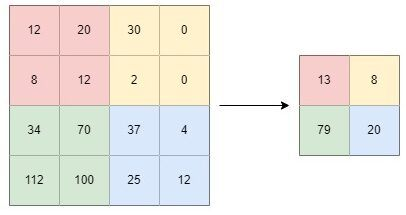
\includegraphics[width = \textwidth]{Average_Pooling.jpg}%
		\caption{Average Pooling Layer with Kernel 2x2 and Stride 2}
		\label{fig:fig_average_pooling}
	\end{minipage}
	%https://www.baeldung.com/cs/neural-networks-pooling-layers
\end{figure}
%TODO: Bring more mathematical expressions in the mix
<<<<<<< HEAD
\begin{align}
	MaxPooling(X)_{i,j,k} = \max_{m,n}X_{i\cdot s_x + m, j \cdot s_y+n,k}
\end{align}
\begin{align}
	AveragePooling(X)_{i,j,k} =\frac{1}{f_x\cdot f_y}\sum_{m,n} X_{i\cdot s_x + m, j \cdot s_y+n,k}
\end{align}

%Fully Connected Layer
The Fully Connected(FC) layer connects all neurons from the previous layer to all neurons in the subsequent layer, enabling the network to make high-level decisions based on the learned features. The neurons of this layer are organized in a array form. This layer is used to optimize objectives as class scores.\\%TODO: mehr infos sehr kurze beschreibung 


%TODO: Übergang fehlt 
%AlexNet
AlexNet is a pioneering CNN architecture that played a pivotal role in advancing the field of deep learning and computer vision \cite{Alzubaidi2021}. Alex net won the Image Net Large Scale Visual Recognition Challange(ILSVRC) in 2012 it introduced several groundbreaking concepts, including deep architecture  with multiple convolutional and fully connected layers, ReLU activation functions, dropout for regularization, and GPU acceleration for faster training. Its success highlighted the potential of deep neural networks for image classification tasks, influencing the design of subsequent CNN architectures and shaping the direction of modern deep learning research.
%TODO: Not sure if this section is needed but we will see should probably be removed or i find a way to get on from this text could be connected through Image Net reference

%Transfere Learning 
Due to our lack of training data a possible methode of enhancing our network is using transfer learning. This method is a common and effective strategy to train a network on a small data set. By pretraining the network on extremely large datasets like ImageNet with 1.4 million images and 1000 classes, trying to learn generic features that can be shared among networks \cite{Yamashita2018}.This is a unique advantage of deep learning that makes itself useful in various domain tasks with small datasets. Despite the popularity of transfer learning in medical imaging there hasn't been a lot of work studying of its effects. Usually transfer learning is performed by taking a standard IMAGENET architecture with pretrained weights and then fine tuning its parameters on the dataset which the network is supposed to detect.
%When comparing medical datasets with IMAGENET we can see that medical images usually range from a few hundred to a couple hundred thousands  (not sure if i want to go in this direction)
\cite{NEURIPS2019_eb1e7832} shows on two large scale medical image networks that the gain of transfer learning on those networks is marginal. It also shows that transfer usually helps large scale models, with small models showing little difference. Therefore we wont use transfer learning to enhance our network.

% early stopping / overfitting 
When training a CNN with to little data we usually need to make use of the method of early stopping. This technique is used in machine learning to prevent overfitting during model training. overfitting occurs in machine learning when a model learns to perform well on the training data, capturing noise and irrelevant patterns, but usually performs poor on new unseen data. This indicates that the model has memorized the training data instead of learning the underlying patterns, leading to reduced generalization ability and diminished predictive accuracy on real-world examples. Early stopping involves monitoring the model's performance on a validation dataset and stopping training when the performance on a validation dataset starts to degrade. By preventing excessive training; early stopping helps the model generalize better to new data and improves its ability to make accurate prediction on new data and improves its ability to make accurate predictions.
This technique strikes a balance between training optimal performance and avoiding the point where the model starts memorizing noise in the training data. %letzter satz vlt wecklassen
%TODO: maybe add a part about overfitting (would be smart)
%Since our data set is quite small we needed to find a way to augment our data in a way that we can get more training data to generalize our network without running in the hurdle of overfitting or early stopping. 


%Batch Normalization
To ease the training process we typically normalize the initial values of our parameters by initializing them with zero mean. By training our data we would usually lose this normalization, which slows down training and amplifies changes as the network becomes deeper. %TODO: passender übergang muss gefunden werden 
 To remove those effects and therefore enhance the training stability and convergence of deep neural networks, batch normalization\cite{Ioffe2015} can be employed. By standardizing the inputs within each mini-batch during training , this technique mitigates gradient related issues and accelerates convergence. Additionally it acts as a form of regularization, curbing overfitting. With this metohde we are able to use higher learning rates and pay less attention to the initialization parameters \cite{Ruder2016}.  
 %TODO: read IOffe2015 again and maybe add some more informations also there might be more papers to cite 
 
 
%TODO:Activation functions 
To calculate the output from the weighted sum of the inputs from a node an activation function is needed.Those functions are used to map the input into the required number range like a value between 0 and 1 or 1 and -1.  The choice of the activation function has a large impact on the capability and performance of the neural network. It can ensure a better detection of complicated patterns and even accelerate the learning process \cite{Khan2020}. Comonly used functions are ... \cite{Mishkin2017} recommends to use ELU non-linearity without batch normalization or ReLU with it.
%ReLU -> not sure if i want to talk about it ->vanishing gradient problem 
%TODO: missing transition to sigmoid and part about sigmoid 
sigmoid
\begin{align}
	y = \frac{1}{1+e^{-x}}
\end{align}

The ReLu function has significant adcantages over a sigmoid function in a neural network. The main advantage is that ReLU function is very fast to calculate. For positive x the ReLU function has a constant gradient of 1 whereas a sigmoid function has a gradient that rapidly converges to zero. This property makes neural networks with a sigmoid activation function slower to train. The occurring phenomen is also known as vanishing gradient problem %TODO: vanishing gradient problem description 
ReLu as an activation function removes this problem because the gradient of ReLU is always one for positive x so that the learningprocess wont be slowed down by a vanishing gradient. 

 

ReLU
\begin{align}
	y = \max(x,0)
\end{align}
However the zero gradient can pose the zero gradient problem %TODO: explain the zer gradient problem
this can be compensated by adding a smaller linear term in x to give the ReLU function a nonzero slope at all points this is solved in the implementation by adding $\alpha(e^x-1)$ for all values smaller than zero. Therefore the gradient of ELU is allways bigger than 0, tending to zero for $x \rightarrow - \infty$.

ELU
\begin{align}
	y = 
	\begin{dcases}
		x \text{, if } x \geq 0 \\
		\alpha(e^x-1) \text{, otherwise}
	\end{dcases}
\end{align}


%TODO: Convolutional Block Attention Module 
Convolution based attention module(CBAM) is a simple yet effective attention module \cite{Woo2018}
%-it is ligthweight and tehrefore it can be implemented into any CNN 
%- consists of channel attention module and spatial attention module which are used to refine the input features 
%-( investigate a different aspect of the architecture design, attention)
%read paper \cite{Woo2018}


%network in Network 
%Bayesan Approaches
%dropout

=======
%Fully Connected Layer
The fully connected layer connects all neurons from the previous layer to all neurons in the subsequent layer, enabling the network to make high-level decisions based on the learned features. The neurons of this layer are organized in a array form. This layer is used to optimize objectives as class scores.\\
>>>>>>> parent of e570a91 (added a lot of text to the latex file)
%Data Augmentation
A big issue in the space of medical imaging is the lack of training data. When training a CNN with to little data we either have to stop early and don't get a optimal accuracy for the network. If we would further train the network with the same samples the network would overfit and lose its validity  
therefore we nee to find a way to augment the data so that it still has the same meaning for a person. The concept of data augmentation is well spread in the medical imaging field 
to use data augmentaiton techniques like rotation 

<<<<<<< HEAD
A big issue in the field of medical imaging is the lack of training data. Due to the fact that just trained staff is capable of labeling the images it is expensive to label the data, also a lack of time from the staff can be an issue. But even with time and money the biggest issue in medical imaging is the lack off data. Since ... %TODO: Daten schutz and stuff maybe this part is unnecessary since i already wrote about it berfore 


 
 
 
%imbalanced data in medical imaging   
 Commonly, biological data tends to be imbalanced, often negative samples are much more numerous than positive ones \cite{Alzubaidi2021}. When training a Network with imbalanced data, the network is prone to to bias towards the major classes, since it priorizes learning the features for detecting those classes. This also means that the network does not get enough exposure to detect minor features and therefore cant learn its distinctive features. All this leads to a higher number of false negatives. With the network trying to capture the minor features it can run into issue of overfitting the network %TODO: here could be the overfitting part if i really want it also the last sentence needs a sentence before with more intell probably i will do it earlyer
 
  S... In our case we have a lack of data that is labeled with the severity level of 4 and 5. This holds a major issue. Since level 4 and 5 scans are in need of a re-scan. Thus we want to have a high accuracy score for detecting these classes to be sure that we wont unnecessarily re-scan patients since we don't want to expose them unnecessary to radiation.%TODO: ausschmücken informationsdichte ist zu hoch 
 
 If we would further train the network with the same samples the network would overfitt and lose its validity  To prevent overfitting from happening we need to implement methods to augment the data, to have more of it to learn from. Since the scans have a depth of 110 layers there is a possibility of taking some of those layers to train on, with this process we need to be carefull how many slices we take since slices that lay close to each other might look to similar so that the network might tend do overfitt faster. Therefore we just take 8 slices which we do based on the decision in \cite{Walle2023}.%TODO:Go deeper
  There are also a few other ways, a very common technique to augmentation data, is to rotate them. Those images add stability to the algorithm since radius and tibia can lay in various places and still need to be detected the same way. To augment our data we took %TODO: depending on what i will do with my data
Another common augmentation technique is to add  a small amount of gaussian noise to the image, so small, that the image still looks the same way to a human.Since it would still be interpreted the same way from a doctor it also needs to be interpreted the same way by the Network. This ensures that the network does not focus on specific data points. This leads to a more robust network.
%TODO: do i want to add croppend images so that the network can learn on more examples this can work when the bone lies in different fields of the image but i have to see if that is possible??


%Data.

%TODO: \cite{Szegedy_2015_CVPR} GoogleNet

\begin{center}
	\begin{tabular}{||c|c|c||}
		
		 Motion Grade&  Tibia rounded& Radius rounded  	\\
		\hline
		\hline
		1 &  334&  139   \\
		\hline
		2 &  97&  169 	\\
		\hline
		3 &  42&  233   \\
		\hline
		4 &  24&  62   \\
		\hline
		5 &  2&  8 \\
		\hline
	\end{tabular}
\end{center}

The data was provided by the osteology department of the ``Unfall Klinikum Eppendorf'' and Labeled by 3 doctors of the department (need to check wether thats correct). The labeled data contained 500 Scans of the radius and 500 scans of the tibia. In  51.1 \% of all scans the doctors had a consens, 57\% for grading the tibia and 45.2\% for grading the radius. 

In 7.4\% a rescan could have occured 4.6\% for tibia and 10.2 percent for the radius. This is hard to compare since we have a way bigger amount of values in the domain of 3 and 4 for the radius compared to the tibia. If we therefore link the amount of values that where the rounded gathered rating was 3 or 4 with the possibility of a rescan we get : 34\% for tibia and 27.9\% overall this concludes to  %TODO this text need to be rewritten because of lack of motivation



%TODO: make a patr about this it sounds very interresting it pairs well with CBAM most of recent network engineering methods mainly target on three factors depth [19,9,10,5], width [10,22,6,8], and cardinality [7,11], we focus on the other aspect, ‘attention’, 
%to incorporate: global average pulled features are  suboptimal features in order to infer fine channel attention and we suggest to use max-pooled features as wel
=======
\begin{align}
 \zb S &= \zb c \zb u
\end{align}

>>>>>>> parent of e570a91 (added a lot of text to the latex file)
\chapter{Experimental Setup}



\chapter{Results}

\chapter{Discussion}

\bibliographystyle{unsrt} %unsrt abbrv
\bibliography{Bibliography}

\end{document}
